\documentclass[compress,blue]{beamer}
\logo{\includegraphics[width=0.12\textwidth]{stout_logo}\hspace{-2pt}}
% \usetheme{default}
%\usetheme{Boadilla}
%\usetheme{Bergen}
\usetheme{Berkeley}
%\usetheme{Goettingen}
%\usetheme{Hannover}
%\usetheme{Luebeck}
% \usetheme{Madrid}
%\usetheme{Montpellier}
%\usetheme{Rochester}
%\usetheme{Warsaw}

% \mode<presentation>
\usepackage{amsmath} \usepackage{graphicx}
\usepackage{amsfonts} \usepackage{amssymb}

\def\QED{{\ \vbox{\hrule\hbox{\vrule height1.3ex\hskip0.8ex\vrule}\hrule}}\par}
\def\ds{\displaystyle}
\newcommand{\pdiff}[2]{\frac{\partial #1}{\partial #2}}
\newcommand{\pdiffsec}[2]{\frac{\partial^2 #1}{\partial^2 #2}}
\newcommand{\diff}[2]{\frac{d #1}{d #2}}

%%%%%%%%%%%%%%% EITHER DEVELOP A CATCHY TITLE OR USE THE INDUSTRY SPONSOR NAME %%%%%%%%%%%%%%%
\title{The District Company: Predictive Analytics for Sales and Marketing}
%%%%%%%%%%%%%%% IF THE COMPANY NAME DOES NOT APPEAR, PLACE IT AFTER THE LIASON'S NAME %%%%%%%%%%%%%%%
%%%%%%%%%%%%%%% E.G. Steve Jobs, Apple Inc. %%%%%%%%%%%%%%%
\subtitle{Industry Liason: Dustin Jepperson}

%%%%%%%%%%%%%%% ENTER YOUR GROUP MEMBERS HERE %%%%%%%%%%%%%%%
\author{Megan Mortensen, Connor Phu, \\
Brian Dassow, Bella Nordahl}

%%%%%%%%%%%%%%% REPLACE THE BLUE DEVILS LOGO WITH THE COMPANY LOGO IF ONE EXISTS %%%%%%%%%%%%%%%
\titlegraphic{\includegraphics[width=0.33\textwidth]{pic_math_logo}\hspace{0cm}
\includegraphics[width=0.33\textwidth]{DistrictCompanylogo}}

\institute{\textbf{University of Wisconsin Stout} \\
}
\date{April 28, 2016}


\begin{document}

% this prints title, author etc. info from above
\frame{\titlepage}

%\frame{\frametitle{Outline}\tableofcontents[pausesections]}

%%%%%%%%%%%%%%% BELOW IS YOUR SLIDE DECK %%%%%%%%%%%%%%%
%%%%%%%%%%%%%%% CHANGE SLIDE TITLES, ETC. AS YOU DEEM APPROPRIATE %%%%%%%%%%%%%%%
%%%%%%%%%%%%%%%%%%%%%%%%%%%%%%%%%%%%%%%%%%%%%%%%%%%%%%%%%%%
%%%%%%%%%%%%%%% MUST INCLUDE:
%%%%%%%%%%%%%%% (1) Give a statement of the problem and tell why the problem is important
%%%%%%%%%%%%%%% (2) Brief statement of your results
%%%%%%%%%%%%%%% (3) Details about your approach to the problem  
%%%%%%%%%%%%%%% (4) More detailed presentation of your results
%%%%%%%%%%%%%%% (5) Restatement of the problem and the results
%%%%%%%%%%%%%%% (6) Suggested future work
%%%%%%%%%%%%%%% (7) Acknowledgements slide (Leave this slide in the deck, just edit accordingly.)
%%%%%%%%%%%%%%% %%%%%%%%%%%%%%% %%%%%%%%%%%%%%% %%%%%%%%%%%%%%%


\section{Introducing the Problem}

\begin{frame}{Problem Statement}
\setbeamertemplate{itemize items}[circle]
\begin{itemize}
	\item Interpret data to help the company make important business decisions
	\item Look at the correlation between events and concession sales
	\item Create and evaluate surveys to determine what customers want and need
\end{itemize}
\end{frame}

\begin{frame}{Problem Importance or Relevance}
\setbeamertemplate{itemize items}[circle]
	\item They can make business decisions based off our results
	\begin{itemize}
	  \item Know which games and events bring in the most profit in concession
	  sales
	  \item Know which events do better than others
	  \item Informed about how to best meet the customers' needs
	\end{itemize}
\end{frame}

\section{Data Analysis}

\begin{frame}{Events}
\vspace{0cm}
\begin{rows}
\row{\textwidth}
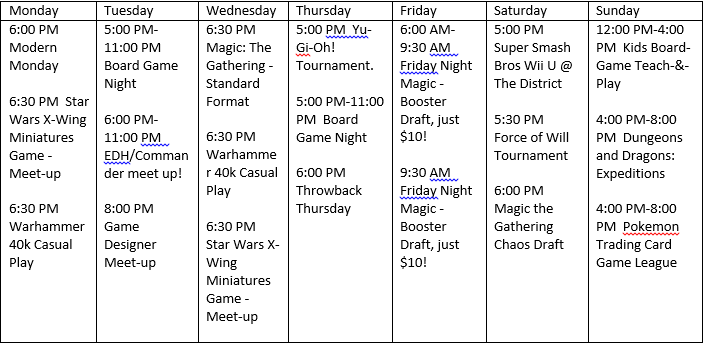
\includegraphics[width=8cm,height=3cm]{DistrictCompanyEventSchedule}
\row{\textwidth}
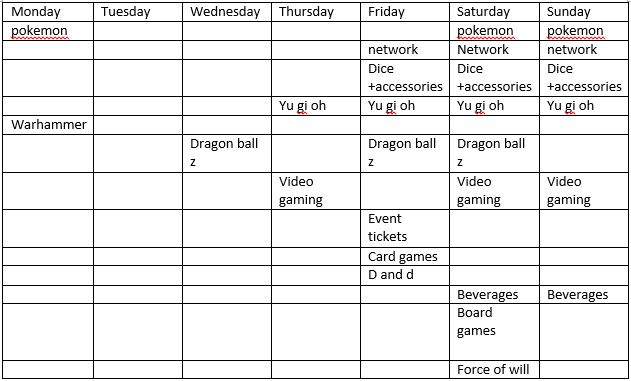
\includegraphics[width=8cm,height=3cm]{MegansFindings}
\end{rows}
\newline
Suggestion: Market Wednesday Warhammer event
\end{frame}

\begin{frame}{Total Monthly Revenue}
\vspace{0cm}
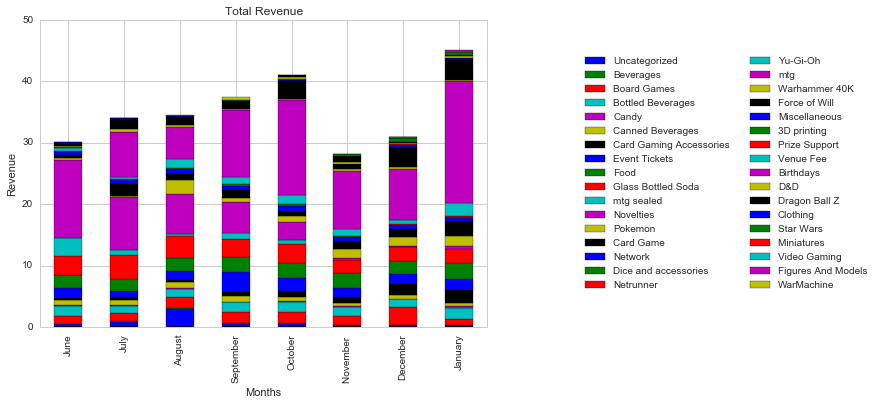
\includegraphics[width=9cm,height=5cm]{TotalMonthlyRevenue}
\newline
Suggestion: Market sales for holidays, especially Dragon Ball Z and Board and
Card Games
\end{frame}


\section{Regressions}

\begin{frame}{Correlations with Food and Different Beverages}
\begin{rows}
\row{\textwidth}
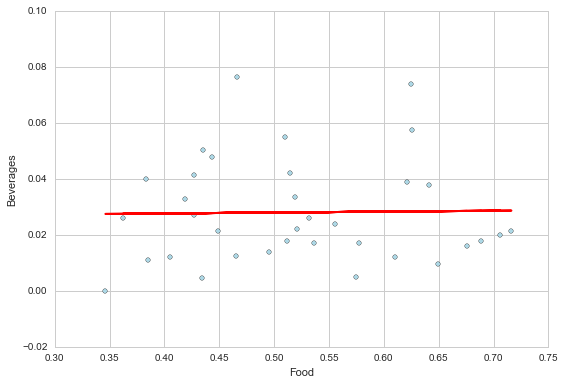
\includegraphics[width=3.25cm,height=3.25cm]{Bev&Food}
\hspace{1.5cm}
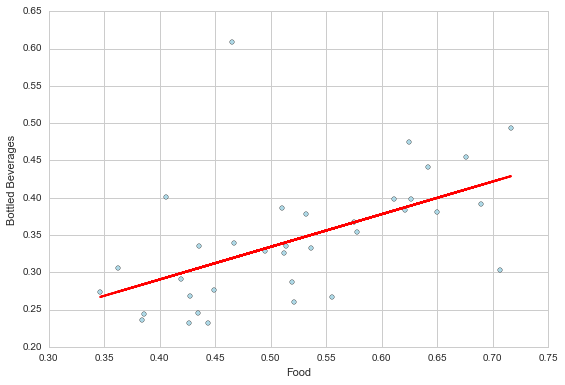
\includegraphics[width=3.25cm,height=3.25cm]{Bottled&Food}
\row{\textwidth}
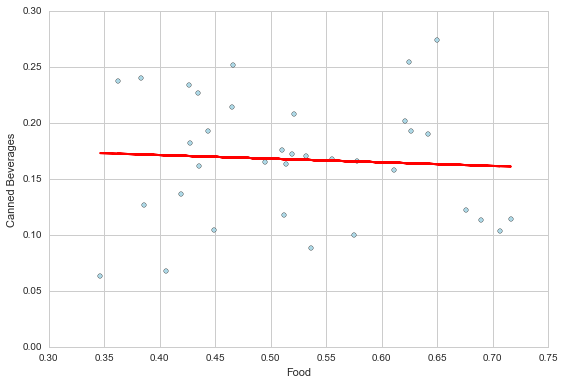
\includegraphics[width=3.25cm,height=3.25cm]{Canned&Food}
\hspace{1.5cm}
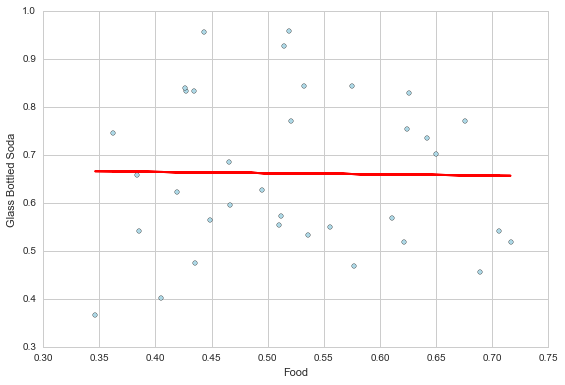
\includegraphics[width=3.25cm,height=3.25cm]{Glass&Food}
\end{rows}
\newline
Suggestion: Encourage customers to buy beverages other than Bottled Beverages
when buying food
\end{frame}

\begin{frame}{Multiple Regression Weights}
\begin{center}
\tiny
\begin{center}After D\&D By Weeks\end{center}
\vspace{0.3cm}
\tiny
\begin{tabular}{| c | c | c | c | c | c |}
 $x/y$ down & MTG Combined  & D\&D  & Novelties  & Event Tickets  & Board
 Games\\ 
 \hline 
 \hline
 Beverages & {\color{blue}-0.004} & {\color{blue}0.017} &
 {\color{blue}0.024} & {\color{blue}-0.014} & {\color{blue}-0.024} \\
 \hline
 Bottled Beverages & {\color{blue}0.014} & {\color{orange}-0.236} &
 {\color{blue}0.085} & {\color{blue}-0.012} & {\color{blue}0.034} \\
 \hline
 Food & {\color{blue}0.031} & {\color{orange}-0.230} &
 {\color{blue}0.037} & {\color{blue}0.094} & {\color{blue}0.092} \\
 \hline
 Glass Bottle Beverages & {\color{blue}0.023} & {\color{orange}0.261} &
 {\color{orange}0.188} & {\color{blue}0.023} & {\color{blue}0.084} \\
 \hline
 Canned Beverages & {\color{blue}-0.006} & {\color{blue}0.023} &
 {\color{blue}0.023} & {\color{blue}0.084} & {\color{blue}-0.024} \\
 \hline
 Candy & {\color{blue}0.003} & {\color{blue}0.070} &
 {\color{blue}-0.025} & {\color{blue}0.004} & {\color{blue}-0.017} \\
 \hline 
\end{tabular}

\vspace{-.27cm}

\begin{center}

\end{center}
\tiny
\begin{center}Before D\&D By Days\end{center}
\tiny
\begin{tabular}{ c || c | c | c | c | c |}
 $x/y$ down & MTG & D\&D  & Novelties  & Event Tickets  & Board
 Games\\ 
 \hline 
 \hline
 Beverages & {\color{blue}0.001} & {\color{blue}0.010} &
 {\color{blue}0.005} & {\color{blue}-0.004} & {\color{blue}-0.007} \\
 \hline
 Bottled Beverages & {\color{blue}0.020} & {\color{blue}-0.041} &
 {\color{blue}0.030} & {\color{blue}0.052} & {\color{blue}0.088} \\
 \hline
 Food & {\color{blue}0.026} & {\color{orange}0.107} &
 {\color{blue}0.033} & {\color{blue}0.085} & {\color{orange}0.104} \\
 \hline
 Glass Bottle Beverages & {\color{blue}0.032} & {\color{blue}0.089} &
 {\color{orange}0.137} & {\color{blue}0.015} & {\color{orange}0.185} \\
 \hline
 Canned Beverages & {\color{blue}0.003} & {\color{blue}0.023} &
 {\color{blue}0.026} & {\color{blue}0.026} & {\color{blue}0.015} \\
 \hline
 Candy & {\color{blue}0.003} & {\color{blue}0.009} &
 {\color{blue}-0.003} & {\color{blue}0.0001} & {\color{blue}0.002} \\
 \hline 
\end{tabular}
\begin{center}
\begin{tablenotes}
{{\color{green} greater than 1.0},
 {\color{magenta}0.51 to 0.99}, {\color{orange}0.1 to 0.5}, 
 {\color{blue} less than 0.1}}
\end{tablenotes}
\end{center}
\end{center}

\newline
\small
Suggestions: 
\setbeamertemplate{itemize items}[circle]
\begin{itemize}
	\item Market Bottled Beverages and Food more during D\&D events
	\item Market all Food and Drink products better during MTG events
\end{itemize}
\end{frame}

\begin{frame}{Big Data Analysis}
\setbeamertemplate{itemize items}[circle]
\begin{itemize}
  \item Given:
  \setbeamertemplate{itemize items}[circle] 
  \begin{itemize}
    \item Item Name
    \item Category
    \item Amount Sold
    \item Gross Sales
    \item Profit
    \item Tax
  \end{itemize}  
  \item Able to decrease the scope
  \item Data is organized in Data Frames
\end{itemize}
\end{frame}

\begin{frame}{Decrease Scope Explanation}
\vspace{0cm}
\begin{columns}
\column{\textwidth}
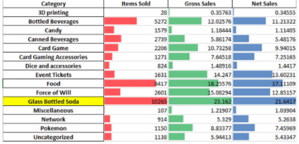
\includegraphics[width=5cm,height=3cm]{FirstPart}
\column{\textwidth}
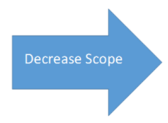
\includegraphics[width=5cm,height=3cm]{Arrow}
\column{\textwidth}
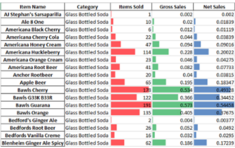
\includegraphics[width=5cm,height=3cm]{LastPart}
\end{columns}
\end{frame}


\begin{frame}{Category Sums}
\vspace{0cm}
\row{\textwidth}
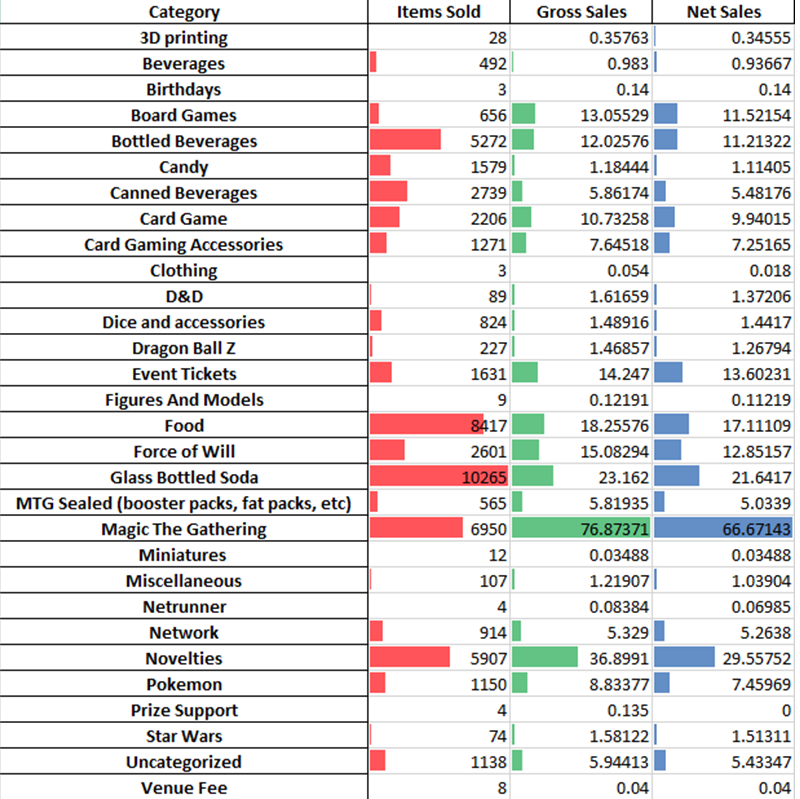
\includegraphics[width=10.5cm,height=7cm]{CategorySums}
\end{frame}


\begin{frame}{Comparisons Between Items Sold and Net Sales}
\begin{rows}
\row{\textwidth}
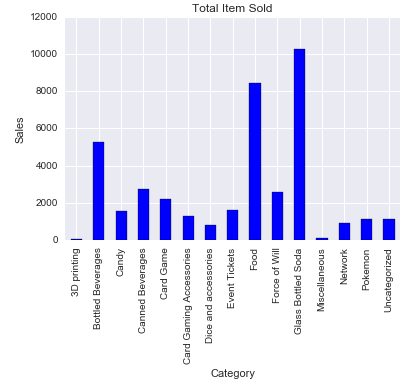
\includegraphics[width=4cm,height=4cm]{TotalItemsSold}
\hspace{1cm}
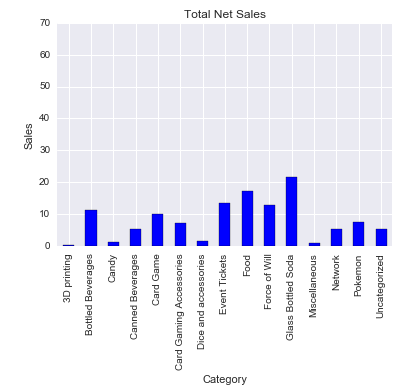
\includegraphics[width=4cm,height=4cm]{TotalNetSales}
\end{rows}
\newline
Suggestion: Raise prices of Glass Bottled Soda, Food, and Bottled Beverages
\end{frame}



\section{Acknowledgements}

\begin{frame}{Acknowledgements}
\setbeamertemplate{itemize items}[circle]
\begin{itemize}
\item PIC Math is a program of the Mathematical Association of America (MAA) and the Society for Industrial and Applied Mathematics (SIAM).  Support is provided by the National Science Foundation (NSF grant DMS-1345499).

\item Advisor: Dr. Keith J. Wojciechowski

\item Project Consultant: Dustin Jepperson

\item The District Company
\end{itemize}

\end{frame}


\end{document} 
